% =============================================================================
%  AeroTraj-Ultra — model schematic, hand-written TikZ.
%
%  This is the LaTeX-native version of docs/figures/architecture_overview.png:
%  the structure is written in TikZ primitives (nodes, arrows, fit-based stage
%  containers, bit-vector pictures) instead of being exported from matplotlib, so
%  it inherits the document's fonts and can be edited like any other LaTeX.
%
%  Build (needs a TeX distribution, e.g. MiKTeX):
%      pdflatex model_schematic_tikz.tex
%  which produces a tight PDF (standalone class) for \includegraphics.
%
%  Requires: tikz with the libraries below. No external images.
% =============================================================================
\documentclass[border=6pt]{standalone}

\usepackage[T1]{fontenc}
\usepackage{lmodern}
\usepackage{amsmath,amssymb}
\usepackage{tikz}
\usetikzlibrary{positioning, arrows.meta, fit, backgrounds, calc, shapes.geometric}

% ---------------------------------------------------------------- style system
\definecolor{roleInp}{HTML}{FFF2CC}
\definecolor{roleInpEdge}{HTML}{D6B656}
\definecolor{roleEnc}{HTML}{DAE8FC}
\definecolor{roleEncEdge}{HTML}{6C8EBF}
\definecolor{roleDec}{HTML}{D5E8D4}
\definecolor{roleDecEdge}{HTML}{82B366}
\definecolor{rolePri}{HTML}{FFE6CC}
\definecolor{rolePriEdge}{HTML}{D79B00}
\definecolor{roleOut}{HTML}{F8CECC}
\definecolor{roleOutEdge}{HTML}{B85450}
\definecolor{roleCtx}{HTML}{D5F5F5}
\definecolor{roleCtxEdge}{HTML}{3F9A9A}

\tikzset{
  blk/.style   = {draw, rounded corners=2.5pt, line width=0.75pt, align=center,
                  inner sep=4.5pt, font=\small, minimum height=1.05cm,
                  text width=4.5cm},
  inp/.style   = {blk, fill=roleInp, draw=roleInpEdge},
  encb/.style  = {blk, fill=roleEnc, draw=roleEncEdge},
  decb/.style  = {blk, fill=roleDec, draw=roleDecEdge},
  prib/.style  = {blk, fill=rolePri, draw=rolePriEdge},
  outb/.style  = {blk, fill=roleOut, draw=roleOutEdge},
  ctxb/.style  = {blk, fill=roleCtx, draw=roleCtxEdge},
  stage/.style = {draw, dashed, rounded corners=4pt, line width=0.7pt,
                  draw=black!35, inner sep=7pt},
  stagetitle/.style = {font=\small\bfseries, text=black!75, inner sep=2pt},
  ar/.style    = {-{Latex[length=2.1mm, width=1.5mm]}, draw=black!70,
                  line width=0.7pt},
  ard/.style   = {ar, dashed, draw=rolePriEdge},
  arh/.style   = {ar, draw=rolePriEdge},
  small/.style = {font=\scriptsize, text=black!70},
  label/.style = {font=\scriptsize, text=black!60, inner sep=1.5pt},
}

% a row of bit squares, the visual signature of the binary encoding
\newcommand{\bitrow}[3]{% #1 = coordinate, #2 = number of cells, #3 = cell size
  \begin{scope}[shift={#1}]
    \foreach \i in {0,...,\numexpr#2-1\relax}{%
      \pgfmathparse{int(mod(\i,3)==0 || mod(\i,5)==0)}%
      \ifnum\pgfmathresult=1
        \fill[black!80] (\i*#3,0) rectangle ++(#3*0.72,#3*0.72);
      \fi
      \draw[black!55, line width=0.25pt] (\i*#3,0) rectangle ++(#3*0.72,#3*0.72);
    }
  \end{scope}}

\begin{document}
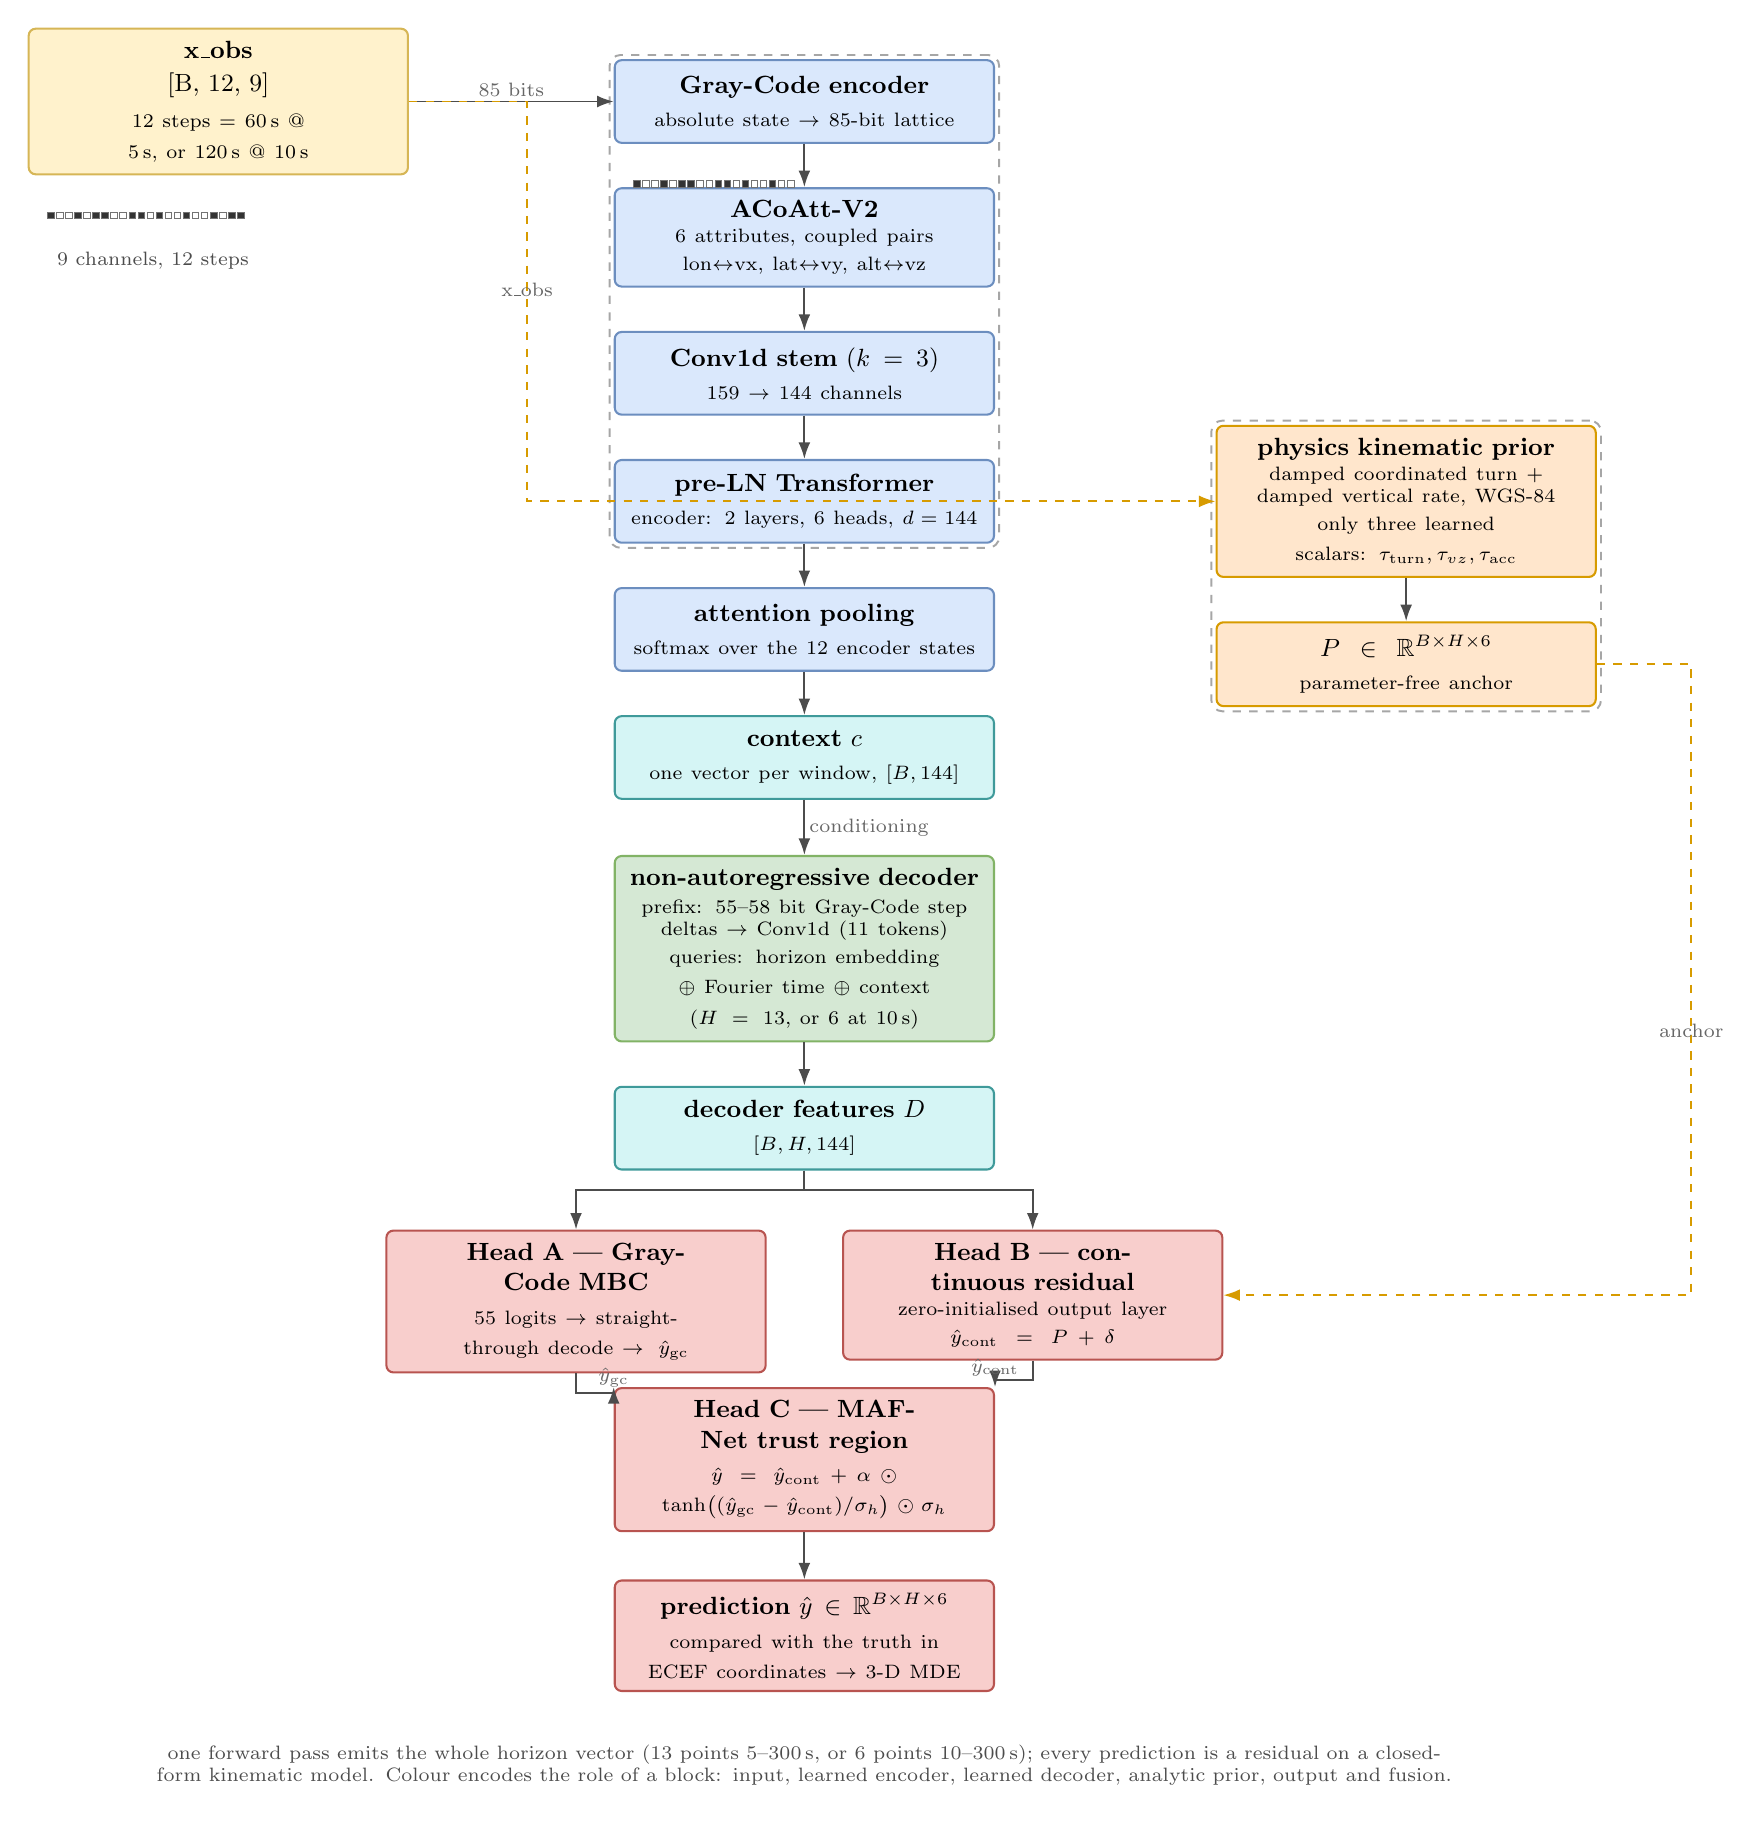
\begin{tikzpicture}

% ============================================================ input + encoder
\node[inp] (x) at (0,0)
  {\textbf{x\_obs}\\[1pt]\small[B, 12, 9]\\[2pt]
   \scriptsize 12 steps = 60\,s @ 5\,s, or 120\,s @ 10\,s};

\node[encb, right=2.6cm of x] (gc)
  {\textbf{Gray-Code encoder}\\[1pt]
   \scriptsize absolute state $\to$ 85-bit lattice};

\node[encb, below=0.55cm of gc] (acoat)
  {\textbf{ACoAtt-V2}\\[1pt]
   \scriptsize 6 attributes, coupled pairs\\[-1pt]
   \scriptsize lon$\leftrightarrow$vx, lat$\leftrightarrow$vy, alt$\leftrightarrow$vz};

\node[encb, below=0.55cm of acoat] (conv)
  {\textbf{Conv1d stem} ($k=3$)\\[1pt]
   \scriptsize 159 $\to$ 144 channels};

\node[encb, below=0.55cm of conv] (trf)
  {\textbf{pre-LN Transformer}\\[1pt]
   \scriptsize encoder: 2 layers, 6 heads, $d=144$};

\node[encb, below=0.55cm of trf] (pool)
  {\textbf{attention pooling}\\[1pt]
   \scriptsize softmax over the 12 encoder states};

\node[ctxb, below=0.55cm of pool] (ctx)
  {\textbf{context $c$}\\[1pt]
   \scriptsize one vector per window, $[B,144]$};

% ============================================================ decoder + prior
\node[decb, below=0.7cm of ctx] (dec)
  {\textbf{non-autoregressive decoder}\\[2pt]
   \scriptsize prefix: 55--58 bit Gray-Code step deltas $\to$ Conv1d (11 tokens)\\[-1pt]
   \scriptsize queries: horizon embedding $\oplus$ Fourier time $\oplus$ context
   ($H=13$, or 6 at 10\,s)};

\node[ctxb, below=0.55cm of dec] (D)
  {\textbf{decoder features $D$}\\[1pt]
   \scriptsize $[B, H, 144]$};

\node[prib, right=2.8cm of trf] (prior)
  {\textbf{physics kinematic prior}\\[1pt]
   \scriptsize damped coordinated turn $+$ damped vertical rate, WGS-84\\[-1pt]
   \scriptsize only three learned scalars: $\tau_{\text{turn}}, \tau_{vz}, \tau_{\text{acc}}$};

\node[prib, below=0.55cm of prior] (P)
  {\textbf{$P \in \mathbb{R}^{B\times H\times 6}$}\\[1pt]
   \scriptsize parameter-free anchor};

% ==================================================================== heads
\node[outb, below=0.75cm of D, xshift=-2.9cm] (headA)
  {\textbf{Head A — Gray-Code MBC}\\[1pt]
   \scriptsize 55 logits $\to$ straight-through decode $\to \hat{y}_{\text{gc}}$};

\node[outb, below=0.75cm of D, xshift=2.9cm] (headB)
  {\textbf{Head B — continuous residual}\\[1pt]
   \scriptsize zero-initialised output layer\\[-1pt]
   \scriptsize $\hat{y}_{\text{cont}} = P + \delta$};

\node[outb, below=2.75cm of D] (headC)
  {\textbf{Head C — MAF-Net trust region}\\[1pt]
   \scriptsize $\hat{y} = \hat{y}_{\text{cont}} + \alpha \odot
   \tanh\!\big((\hat{y}_{\text{gc}} - \hat{y}_{\text{cont}})/\sigma_h\big) \odot \sigma_h$};

\node[outb, below=0.6cm of headC] (yhat)
  {\textbf{prediction $\hat{y} \in \mathbb{R}^{B\times H\times 6}$}\\[1pt]
   \scriptsize compared with the truth in ECEF coordinates $\to$ 3-D MDE};

% ================================================================ bit vectors
\bitrow{($(x.south west)+(0.25,-0.55)$)}{22}{0.115}
\node[small, anchor=north west] at ($(x.south west)+(0.25,-0.85)$)
  {9 channels, 12 steps};
\bitrow{($(gc.south west)+(0.25,-0.55)$)}{18}{0.115}

% ============================================================ stage containers
\begin{scope}[on background layer]
  \node[stage, fit=(gc)(acoat)(conv)(trf), label={[stagetitle]above:%
    Trajectory embedding \;·\; Gray-Code + ACoAtt-V2}] (stageEnc) {};
  \node[stage, fit=(prior)(P), label={[stagetitle]above:Physics prior}] (stagePri) {};
\end{scope}

% ==================================================================== arrows
\draw[ar] (x) -- (gc) node[label, midway, above] {85 bits};
\draw[ar] (gc) -- (acoat);
\draw[ar] (acoat) -- (conv);
\draw[ar] (conv) -- (trf);
\draw[ar] (trf) -- (pool);
\draw[ar] (pool) -- (ctx);
\draw[ar] (ctx) -- (dec) node[label, midway, right] {conditioning};
\draw[ar] (dec) -- (D);

\draw[ard] (x.east) -- ++(1.5,0) |- (prior.west) node[label, pos=0.25, above] {x\_obs};
\draw[ar] (prior) -- (P);
\draw[ard] (P.east) -- ++(1.2,0) |- (headB.east) node[label, pos=0.3, above] {anchor};

\draw[ar] (D.south) -- ++(0,-0.25) -| (headA.north);
\draw[ar] (D.south) -- ++(0,-0.25) -| (headB.north);
\draw[ar] (headA.south) -- ++(0,-0.25) -| (headC.north west)
  node[label, pos=0.55, above] {$\hat{y}_{\text{gc}}$};
\draw[ar] (headB.south) -- ++(0,-0.25) -| (headC.north east)
  node[label, pos=0.55, above] {$\hat{y}_{\text{cont}}$};
\draw[ar] (headC) -- (yhat);

% ==================================================================== caption
\node[small, below=0.55cm of yhat, text width=17cm, align=center]
  {one forward pass emits the whole horizon vector (13 points 5--300\,s, or 6 points
   10--300\,s); every prediction is a residual on a closed-form kinematic model.
   Colour encodes the role of a block:
   input, learned encoder, learned decoder, analytic prior, output and fusion.};

\end{tikzpicture}
\end{document}
